\chapter{Plots}\label{ch:plots}
\section{A function}
Some text before the first plot. % TYPO-ANCHOR
\begin{figure}[htbp]
  \centering
  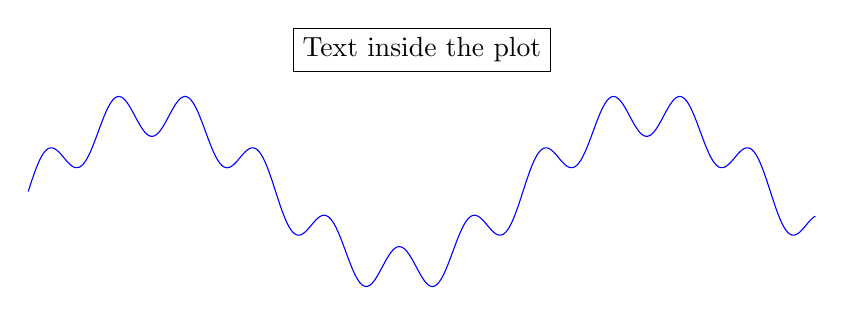
\begin{tikzpicture}
    \draw[domain=0:10,samples=400,blue] plot (\x,{sin(\x r)+0.3*sin(7*\x r)});
    \node[draw] at (5,1.8) {Text inside the plot};
  \end{tikzpicture}
  \caption{A plot}\label{fig:plot}
\end{figure}
An inline picture \tikz \draw (0,0) circle (1ex); in a sentence, and one on a baseline:
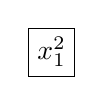
\begin{tikzpicture}[baseline=(n.base)]\node[draw](n){$x_1^2$};\end{tikzpicture} continues.
\todo{A todo note in the margin.}

\begin{figure}[htbp]
  \centering
  \begin{tikzpicture}
    \begin{axis}[width=7cm,height=5cm,xlabel={$x$},ylabel={$f(x)$}]
      \addplot[domain=0:3,samples=60]{x^2};
      \addplot+[only marks] coordinates {(0,1) (1,2) (2,3)};
    \end{axis}
  \end{tikzpicture}
  \caption{An axis}\label{fig:axis}
\end{figure}
\begin{figure}[htbp]
  \centering
  \begin{tikzpicture}
    \begin{axis}[width=6cm,height=4cm]
      \addplot table {data/points.dat};
    \end{axis}
  \end{tikzpicture}
  \caption{Measured points}\label{fig:table}
\end{figure}
See Figure~\ref{fig:axis} and Section~\ref{sec:diagrams}.
